\chapter{Ethereum Transaction Graph Analysis}\label{chap:3}

In this chapter we apply node2vec to obtain structural information from Ethereum network transaction graph. Given the large amount of data that is stored in the blockchain, we make use of the Google BigQuery service to extract only a small relevant subset of nodes and reconstruct transaction graph. After that the node2vec was used to embed this graph into a low-dimensional vector space. The space of embeddings is used to clusterize Ethereum addresses.

\section{Obtaining the Data}
We used Google's BigQuery service to obtain only interesting subset of data through querying block-chain data with SQL. Google maintains the up-to-date complete Ethereum block-chain data on their servers and provides a structural query service to allow data scientists analyze the data without the overhead of downloading gigabytes of data and keeping it up-to-date. 

SQL allows to easily fetch required data. For example, to obtain every transaction that ever happened, we may write:


\begin{lstlisting}{SQL}
SELECT from_address, to_address, value
FROM `bigquery-public-data .crypto_ethereum.transactions`
\end{lstlisting}

\section{Embedding generation}

Using full Ethereum-addresses during the calculation step would require a huge amount of memory. Since the set of network addresses is fixed and known beforehand, we may mitigate this issue by enumerating them at the pre-processing step and using integers as identifiers instead. The mapping (stored as a Python dictionary) can be easily used to resolve the network address when needed.

We use C++ node2vec implementation from SNAP\cite{leskovec2016snap} with the following parameters:

\begin{lstlisting}
node2vec -i:df_connected_numbered.csv -o:node2vec_embedding.txt -d:16 -l:20 -r:5 -k:5 -v
\end{lstlisting}

After the feature representations has been constructed using node2vec, we can use it to estimate roles of involved entities. For the constructed features to be useful and meaningful, we need to keep the number of features as small as possible.

Using unnecessarily high number of dimensions for a feature space inherently implies ambiguities and the observed feature vectors is largely determined by random factors, making it harder or even impossible to come up with a meaningful interpretations for them.

In our case, the optimal size of feature space is appeared to be 3, leading to highly reproducible identifiable patterns in the results as shown on the scatterplot matrix below.

\begin{figure}[H]   \centering
    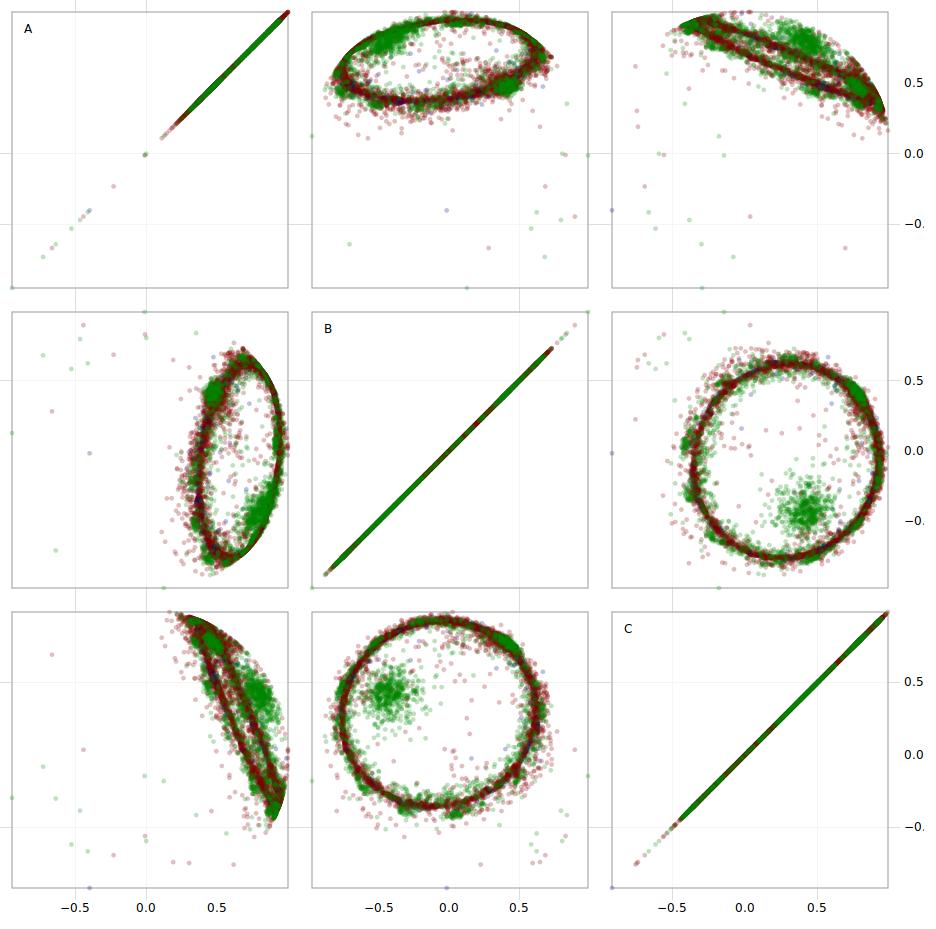
\includegraphics[width=0.7\linewidth]{plots/ScatterplotMatrix1.png}
    \caption{Scatterplot matrix for 3 dimensional embedding. The color of a node is defined by the number of other nodes it connects to: green nodes has at most 2 neighbours, red --- up to 8, others are depicted blue.}
    \label{fig:my_label}
\end{figure}

The nodes on the plot are colored based on the number of connections to another nodes. An interesting pattern can be observed about how the most connected nodes are distributed over the feature space.

\begin{figure}[H]   \centering
    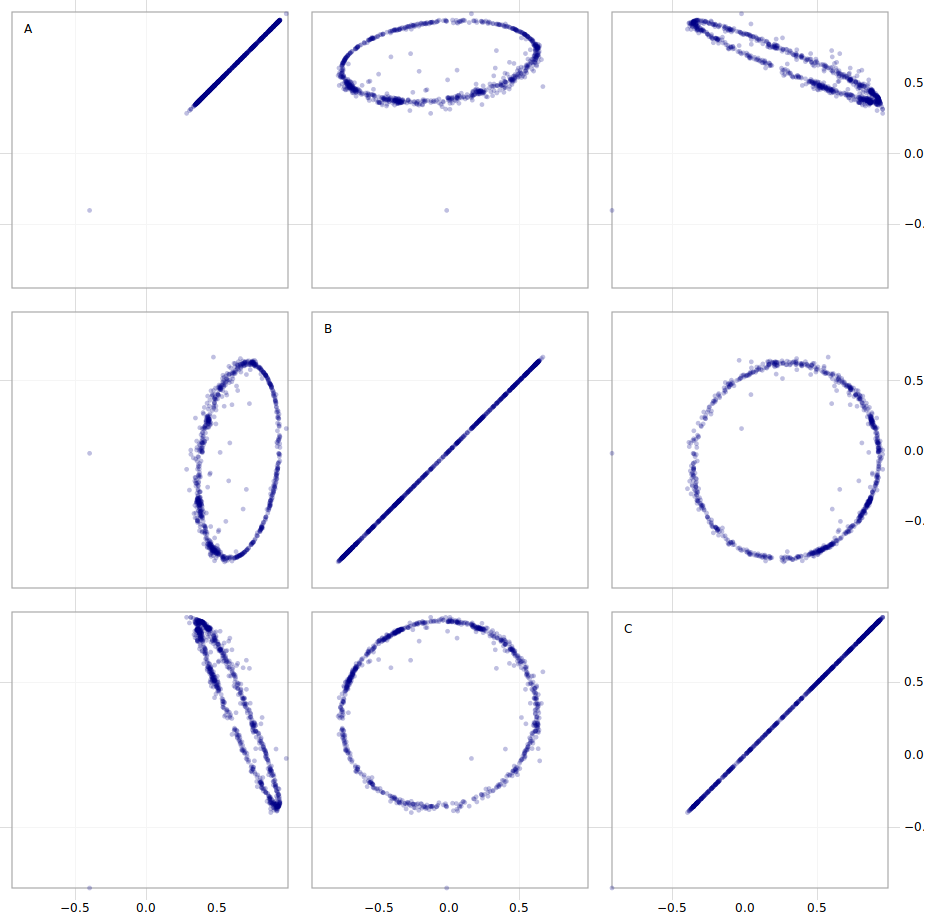
\includegraphics[width=0.7\linewidth]{plots/ScatterplotMatrix2.png}
    \caption{Scatterplot matrix for 3 dimensional embedding showing only nodes with a high number of connections}
    \label{fig:my_label2}
\end{figure}

These nodes are connected to both red nodes with the latter mostly distributed around them in the feature space and green nodes cluster positioned at the center, The green nodes that connects to red ones, in contrast, distributed close to them.

\section{Clustering}

Our data gives the following values of Silhouette coefficients: 
\begin{table}[H]
    \centering
    \begin{tabular}{|l|ccccc|}
        \hline
        Number of clusters   & 5  & 10  & 15 & 20 & 27 \\
        Silhouette coefficient & 0.247 & 0.277 & 0.281 & 0.315 & 0.323 \\
        \hline
    \end{tabular}
    \caption{Silhouette coefficients}
    \label{tab:my_label}
\end{table}

\begin{figure}[H]\centering
  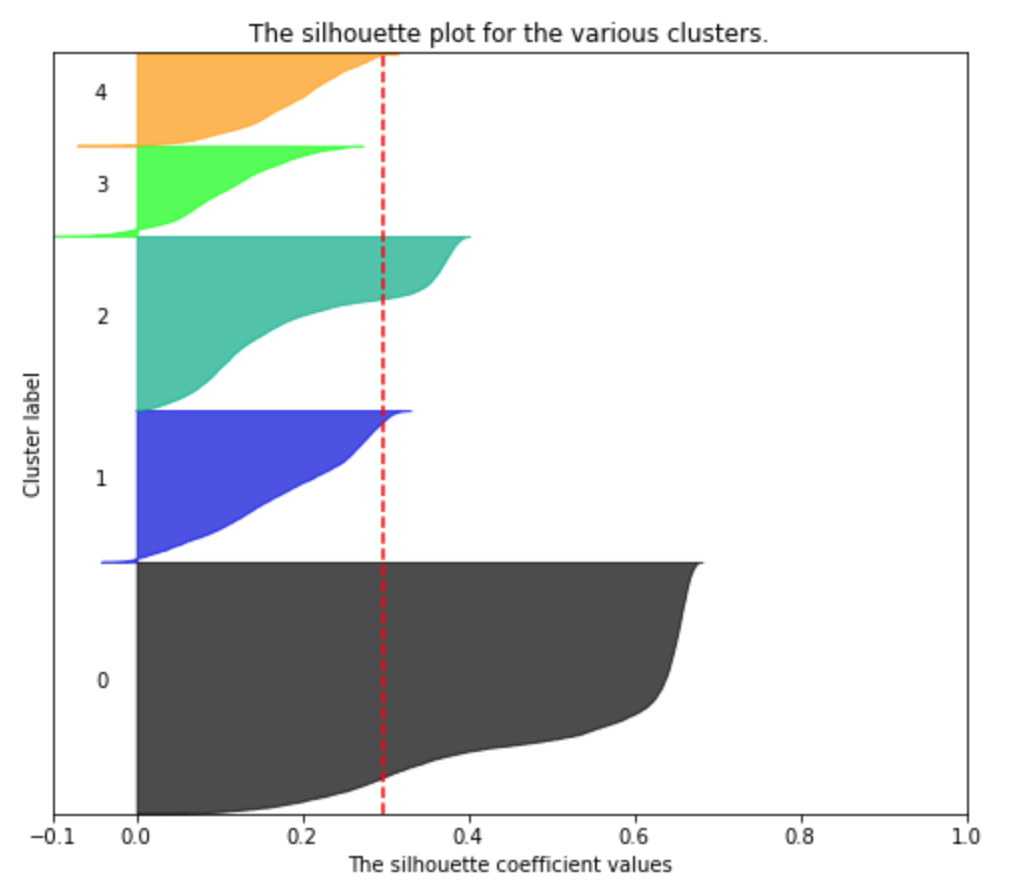
\includegraphics[width=0.6\linewidth]{plots/cluster5.png}
  \caption{Silhouett analysis for K-means clustering on sample data with $n$ clusters = 5.}
\end{figure}

And the optimal number of clusters were 27. The next warning sign was that we had to use t-SNE (t-distributed stochastic neighbor embedding) method to visualize that many clusters. It's a nonlinear dimension-reduction technique, that is designed for visualization high-dimensional data in a low-dimensional space of two dimensions. It maps each high-dimensional object to a two-dimensional point, so that similar objects get mapped to points nearby. Dissimilar objects, instead, map to distant points with high probability.


% The t-SNE algorithm consists of two steps: 
% \begin{itemize}

%     \item Constructing a probability distribution over pairs of high-dimensional objects. For given a set of $N$ objects $x_1, \dots, x_N$ t-SNE first computes probabilities $p_{ij}$, that are proportional to the similarity of objects $x_i$ and $x_j$: \[ 
%           p_{i|j} = \frac{\exp(-\|x_i - x_j \|^2)/2\sigma_i^2}{\sum_{k \neq i}\exp(-\|x_i - x_k \|^2)/2\sigma_i^2},
%     \]
%      \[p_{ij}  = \frac{p_{j|i} + p_{i|j}}{2N}\]

        
%     \item t-SNE aims to learn a $d$-dimensional map $y_1,y_2, \dots , y_N$ that reflects the similarities $p_{ij}$. It measures similarities $q_{ij}$ between two points in the map $y_i$, $y_j$.  The locations of the points $y_i$ in the map are determined by minimizing the  Kullback–Leibler divergence \[ 
%         KL = \sum_{i \neq j} p_{ij} \log \frac{p_{ij}}{q_{ij}}
%     \]
        
% \end{itemize}

% The resulting figure is shown below.

\begin{figure}[H]\centering
  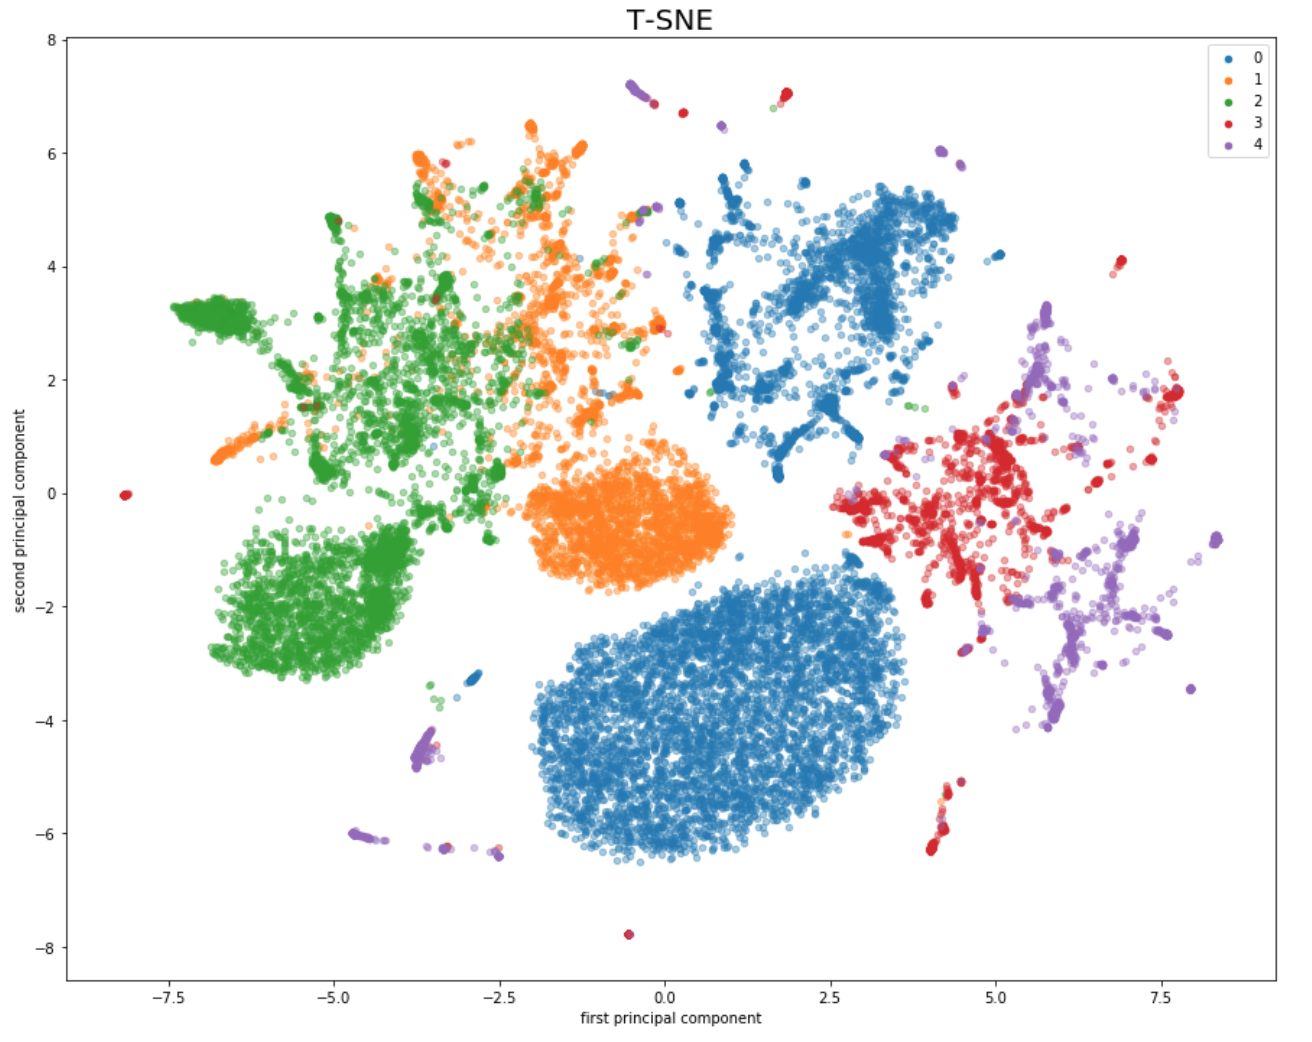
\includegraphics[width=0.8\linewidth]{plots/t-SNE.png}\\
  \caption{16-dimensional data as returned by node2vec mapped to 2-dimensional plane. }
\end{figure}

Here we need to make some notes:

1. On the correct picture we see that there exist simple feature representation, where all addresses are located on the sphere or very close to it. 

2. Addresses were distributed unevenly, mostly in a small circle area on the surface of the sphere. The central part of that area is populated with addresses having just a few transactions. 

3. K-means failed to detect correctly these clusters: the circle cluster of highly active nodes has been recognized as many small clusters instead, leading to a completely incorrect result.

4. Using t-SNE can even further lead to a misperception, since it deforms cluster geometry, making the case of circle cluster broken down into many small ones harder to recognize.

